\chapter{Wi-Fi Brute Force}

Un Brute Force su di una rete Wi-Fi, per prima cosa dobbiamo riuscire a catturare l'handshake che avviene tra il punto di accesso alla rete e il client, in questo handshake possiamo trovare informazioni inerenti alla password.

Per eseguire questo tipo di attacco, un malintenzionato ha addisposizione molti strumenti : Aircrack-ng, Fern, Wifite, AirJack, ecc ecc . Ora andremo a vedere nel dettaglio alcuni di questi strumenti.

\section{Aircrack-ng}

Aircrack-ng\cite{aircrack} è uno strumento utilizzato per valutare la sicurezza delle rete Wi-Fi. Questo tool si compone di una suite di strumenti, ognuno con un proprio scopo :
\begin{itemize}
    \item \textbf{Airmon-ng} utilizzato per impostare l'interfaccia di rete in monitor mode. 
    \item \textbf{Airodump-ng} utilizzato per acquisire i pacchatti di autenticazione Wi-Fi.
    \item \textbf{Aireplay-ng} utilizzato per eseguireun iniezione di frame al fine di generare traffico nella rete.
    \item \textbf{Aircrack-ng} utilizzato per violare le password Wi-Fi.
\end{itemize}

Per eseguire questo tipo dia attacco abbiamo bisogno di una particolare scheda di rete, questa deve supportare la monitor mode\footnote[1]{\textbf{monitor mode} : permette di catturare i pacchetti nella rete senza doversi connettere ad un access point (questa modalità funziona solo con reti wireless)}.

Successivamente dobbiamo andare a configurare la nostra scheda, quindi utilizzeremo il comando riportato qui sotto per individuare la scheda che andremo ad utilizzare.

\begin{lstlisting}[ caption={Configurazione scheda di rete}, style=javaScriptCode]
	root@kali:~# ip a
\end{lstlisting}

\begin{figure}[h!]
    \centering
    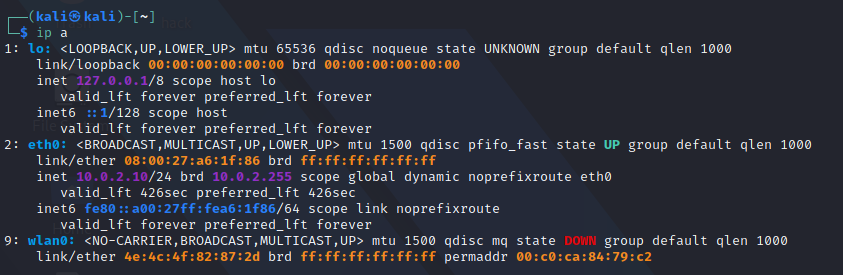
\includegraphics[width=\linewidth]{Immagini/6/aircrack_1.png}
    \caption{Aircrack example}
\end{figure}

\newpage

Una volta individuata la scheda di rete da utilizzare andremo ad eseguire il seguente comando per specificare ad aircrack-ng quale scheda di rete deve utilizzare

\begin{lstlisting}[ caption={Configurazione scheda di rete}, style=javaScriptCode]
	sudo airmon-ng start #nomeschedadirete
\end{lstlisting}

\begin{figure}[ht]
    \centering
    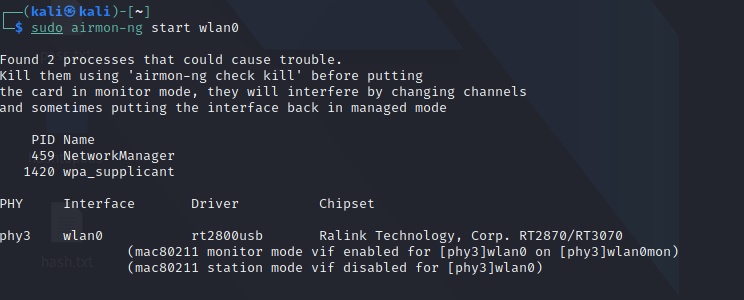
\includegraphics[width=\linewidth]{Immagini/6/aircrack_2.png}
    \caption{Aircrack example}
\end{figure}

Il passo successivo è quello di eseguire una scansione delle reti disponibile, per farlo dobbiamo eseguire il comando :

\begin{lstlisting}[ caption={Scansione delle reti}, style=javaScriptCode]
	sudo airodump-ng wlan0mon
\end{lstlisting}

\begin{figure}[ht]
    \centering
    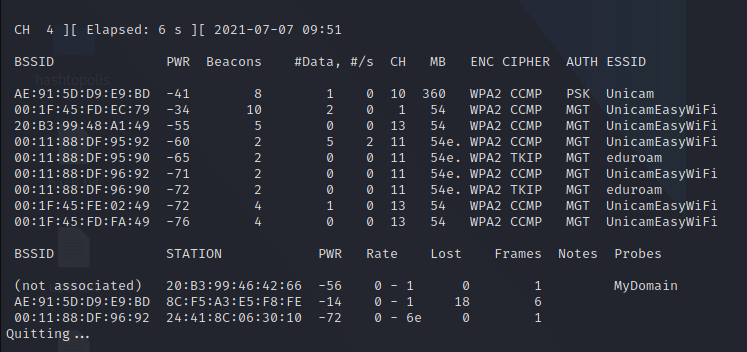
\includegraphics[width=\linewidth]{Immagini/6/aircrack_3.png}
    \caption{Aircrack example}
    \label{fig:Aircrack example}
\end{figure}

\newpage

Dopo aver individuato la rete da attaccare ( in questo caso la rete scelta è Unicam ), dobbiamo salvarci il suo BSSID\footnote[1]{\textbf{BSSID} : Si tratta di un identificatore a 48 bit per il set di servizi di base, è il MAC del lato 802.11 del punto di accesso.} per eseguire un dump dei pacchetti inerenti a quella rete, in modo da poter intercettare i WPA handshake che avvengono tra i client e l'access point. Questi dati verranno memorizzati in un file con estensione .cap\footnote[1]{\textbf{.CAP} : i file con estensione .CAP contengono dati acquisiti dai programmi di tracciamento dei pacchetti. I dati sono in forma grezza, il che significa che vengono salvati nella forma in cui sono stati catturati.} in modo tale da poter eseguire successivamente un Brute Force su questi dati per poterne estrarre la password.

\begin{lstlisting}[ caption={dump dei pacchetti}, style=javaScriptCode]
	sudo airodump-ng --channel 10 --bssid #BSSID_AccessPoint -w #percorso wlan0mon
\end{lstlisting}

\begin{figure}[ht]
    \centering
    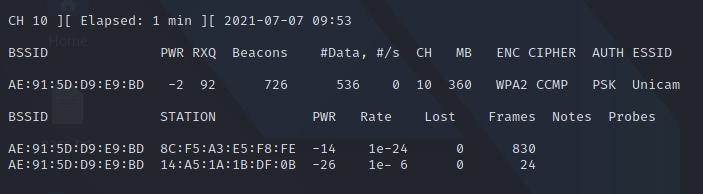
\includegraphics[width=\linewidth]{Immagini/6/aircrack_4.png}
    \caption{Aircrack example}
    \label{fig:Aircrack example}
\end{figure}

Per poter recuperare la password, dobbiamo attendere che venga recuperato il WPA handshake, ma ci potrebbe voler del tempo, quindi una cosa che si può fare è quella di andar a scollegare alcuni utenti dalla rete in modo che cosi debbano ricollegarsi, facendo partire un handshake. Questo è possibile grazie ad aireplay-ng.

\begin{lstlisting}[ caption={aireplay deauth}, style=javaScriptCode]
	sudo aireplay-ng -0 5 -b #BSSID_AccessPoint -h BSSID_Client wlan0mon
\end{lstlisting}

\begin{figure}[ht]
    \centering
    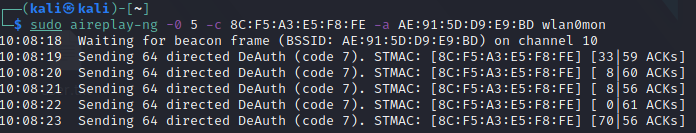
\includegraphics[width=\linewidth]{Immagini/6/aircrack_7.png}
    \caption{Aircrack example}
    \label{fig:Aircrack example}
\end{figure}

Una volta che vediamo che compare la scritta WPA handshake in alto a destra, possiamo chiudere il programma.

\begin{figure}[ht]
    \centering
    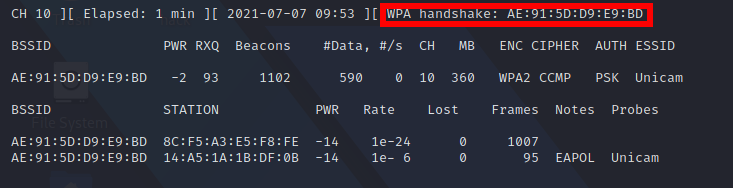
\includegraphics[width=\linewidth]{Immagini/6/aircrack_5.png}
    \caption{Aircrack example}
    \label{fig:Aircrack example}
\end{figure}

Ora che abbiamo recuperato tutti i pacchetti di cui abbiamo bisogno per estrare la password della rete Wi Fi, dobbiamo eseguire un Brute Force su questi dati "grezzi". Per eseguire il Brute Force, possiamo utilizzare il comando aircrack-ng, che permette tramite l'utilizzo di un dizionario, di eseguire un attacco per individuare la password della rete.

\begin{lstlisting}[ caption={aircrack Brute Force}, style=javaScriptCode]
    sudo aircrack-ng -z -b #BSSID_AccessPoint #Path_file_cap -w #Path_Wordlist
\end{lstlisting}

\begin{figure}[ht]
    \centering
    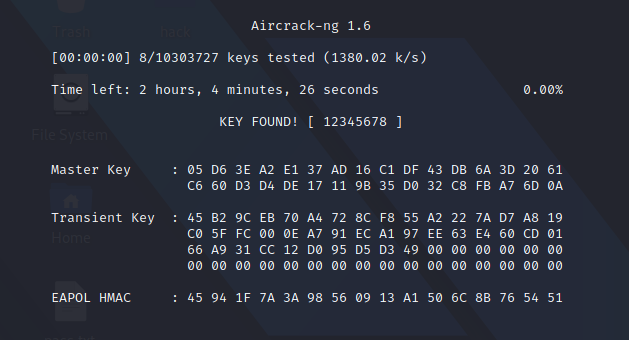
\includegraphics[width=\linewidth]{Immagini/6/ircrack_6.png}
    \caption{Aircrack example}
    \label{fig:Aircrack example}
\end{figure}

\newpage

\section{Fern}

Fern\cite{fern} è un'altro strumento utilizzato per testare la sicurezza delle reti Wi-Fi, come Aircrack. Questo si differenzia per il modo in cui l'utente si interfaccia con il programma, mentre su Aircrack si utilizza un interfaccia a linea di comando, questo strumento ci permette di utilizzare un interfaccia grafica, rendendo l'utilizzo dello strumento più semplice.

\begin{figure}[ht]
    \centering
    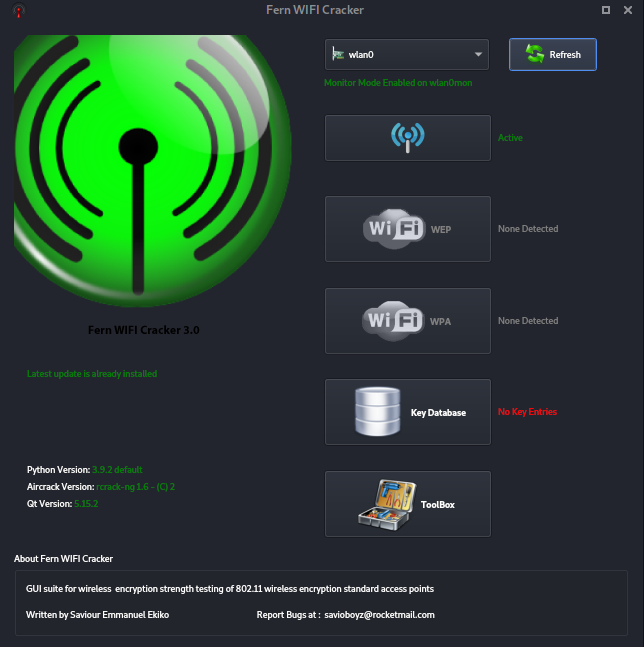
\includegraphics[width=\linewidth]{Immagini/6/fern_1.png}
    \caption{Fern-wifi-cracker}
    \label{fig:Fern example}
\end{figure}

Come possiamo vedere, nella parte superiore possiamo scegliere quale scheda di rete impostare per eseguire la scansione, una volta selezionata la rete possiamo far partire la scansione premendo il tasto sottostante.
\newpage

Una volta avvenuta la scansione, possiamo vedere le reti disponibile suddivise in base al tipo di criptazione, che possono essere o "wifi-wep" o "wifi-wpa", cliccando su uno di questi tasti, possiamo andar a vedere nel dettaglio le reti disponibili. Una volta individuata la rete da attaccare, basterà selezionare la rete, selezionare il dizionario da utilizzare per eseguire l'attacco e premere il tasto \textbf{Attack}.

\begin{figure}[ht]
    \centering
    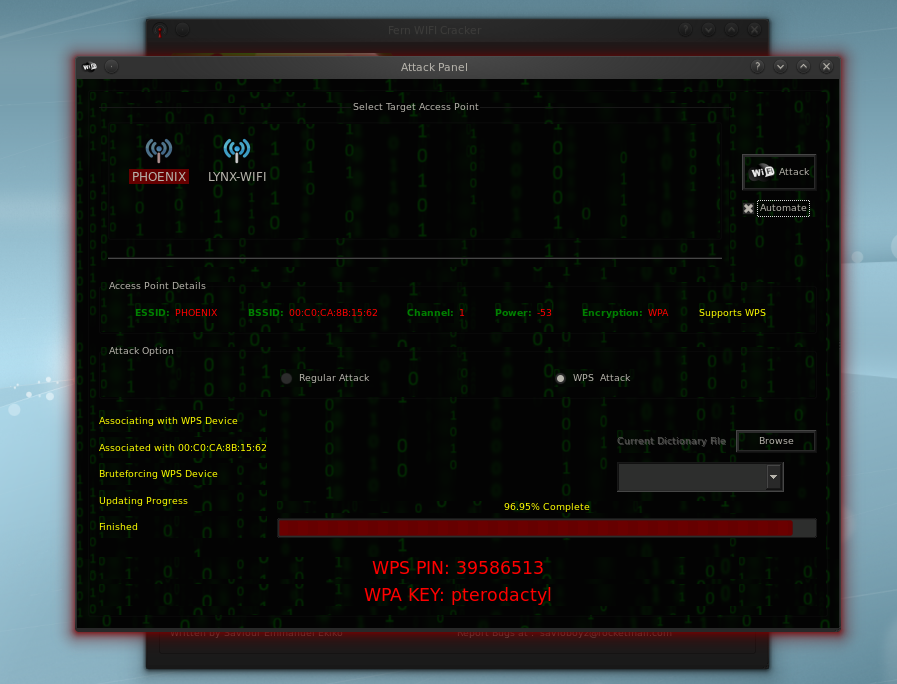
\includegraphics[width=\linewidth]{Immagini/6/fern_3.jpg}
    \caption{Fern-wifi-cracker}
    \label{fig:Fern example}
\end{figure}

\label{chap:conc}
